\begin{problem}
{\textbf{\textsc{Ball Drop}}} Một quả bóng có mật độ đồng nhất \( \rho_b \) được đặt trên mặt nước của một hồ có độ sâu \( d \) và mật độ chất lỏng \( \rho_p < \rho_b \). Một quả bóng giống hệt được nâng lên một độ cao \( h \) trên hồ, và sau đó cả hai quả bóng được thả cùng lúc. Để cả hai quả bóng chạm đáy hồ cùng lúc, điều kiện \( d = nh \) phải được thỏa mãn với một \( n \) không có kích thước nào phụ thuộc vào các giá trị của \( \rho_p \) và \( \rho_b \). Nếu chúng ta định nghĩa \( r \) như sau:
$$r = \frac{\rho_b - \rho_p}{\rho_b}$$
Thì chúng ta có thể biểu diễn \( n \) dưới dạng:
$$n = \frac{Ar^3 + Br^2 + Cr}{Dr^2+Er+F}$$
Trong đó $A, B, C, D, E, F$ là các số nguyên khác không, $\gcd(A,B,C,D,E,F) = 1$, và $A>0$. Tính $A + B + C + D + E + F$?
Bạn có thể giả định rằng các lực duy nhất hiện diện là trọng lực và lực đẩy của nước từ hồ. Quả bóng rơi từ trên không giữ lại năng lượng khi nó vào hồ.
% \FloatBarrier
% \begin{figure}[!htbp]
%     \centering
%     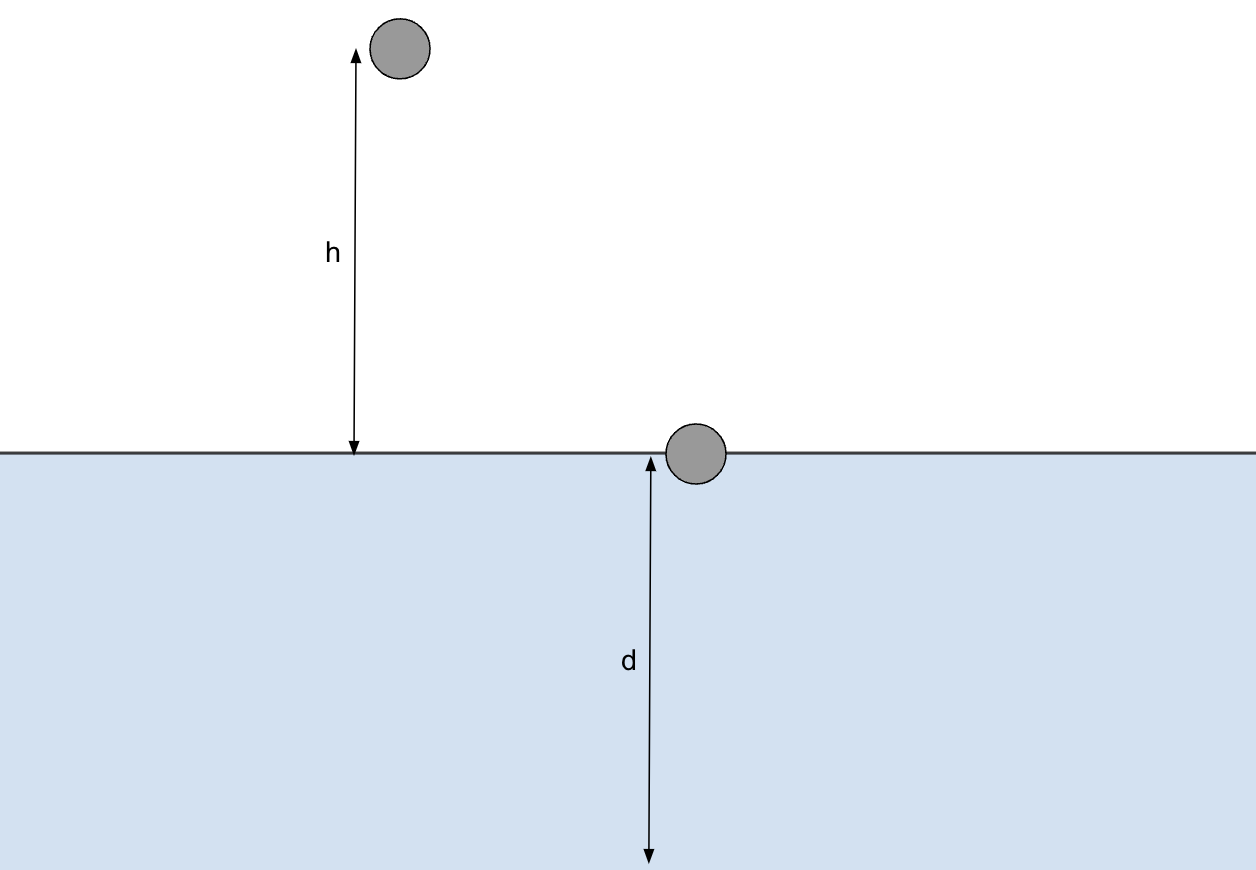
\includegraphics[scale=0.42]{problems/figures/ballDiagram.png}
% \end{figure}
% \FloatBarrier
\end{problem}